\documentclass{ximera}
%\usepackage{todonotes}

\usepackage{tkz-euclide}
\usetikzlibrary{backgrounds} %% for boxes around graphs
\usetikzlibrary{shapes,positioning}  %% Clouds and stars
\usetkzobj{all}
\usepackage[makeroom]{cancel} %% for strike outs
%\usepackage{mathtools} %% for pretty underbrace % Breaks Ximera
\usepackage{multicol}


\newcommand{\RR}{\mathbb R}
\renewcommand{\d}{\,d}
\newcommand{\dd}[2][]{\frac{d #1}{d #2}}
\renewcommand{\l}{\ell}
\newcommand{\ddx}{\frac{d}{dx}}
\newcommand{\zeroOverZero}{$\boldsymbol{\tfrac{0}{0}}$}
\newcommand{\numOverZero}{$\boldsymbol{\tfrac{\#}{0}}$}
\newcommand{\dfn}{\textbf}
\newcommand{\eval}[1]{\bigg[ #1 \bigg]}
\renewcommand{\epsilon}{\varepsilon}
\renewcommand{\iff}{\Leftrightarrow}

\DeclareMathOperator{\arccot}{arccot}
\DeclareMathOperator{\arcsec}{arcsec}
\DeclareMathOperator{\arccsc}{arccsc}


\colorlet{textColor}{black} 
\colorlet{background}{white}
\colorlet{penColor}{blue!50!black} % Color of a curve in a plot
\colorlet{penColor2}{red!50!black}% Color of a curve in a plot
\colorlet{penColor3}{red!50!blue} % Color of a curve in a plot
\colorlet{penColor4}{green!50!black} % Color of a curve in a plot
\colorlet{penColor5}{orange!80!black} % Color of a curve in a plot
                                      \colorlet{fill1}{blue!50!black!20} % Color of fill in a plot
\colorlet{fill2}{blue!10} % Color of fill in a plot
\colorlet{fillp}{fill1} % Color of positive area
\colorlet{filln}{red!50!black!20} % Color of negative area
\colorlet{gridColor}{gray!50} % Color of grid in a plot

\pgfmathdeclarefunction{gauss}{2}{% gives gaussian
  \pgfmathparse{1/(#2*sqrt(2*pi))*exp(-((x-#1)^2)/(2*#2^2))}%
}



\newcommand{\fullwidth}{}
\newcommand{\normalwidth}{}



%% makes a snazzy t-chart for evaluating functions
\newenvironment{tchart}{\rowcolors{2}{}{background!90!textColor}\array}{\endarray}

%%This is to help with formatting on future title pages.
\newenvironment{sectionOutcomes}{}{} 

\author{Emma Smith Zbarsky}
\license{Creative Commons Attribution 3.0 Unported}
\acknowledgement{https://quadbase.org/questions/q14589v1}
\begin{document}

\begin{exercise}

A rancher wants to create a corral with two semi-circular ends and a
rectangular middle. If she has 800 feet of fencing, what is the largest
possible corral she can build.

\begin{image}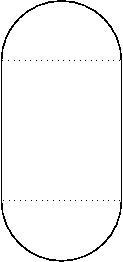
\includegraphics{corral.jpg}\end{image}


\begin{hint}
This is an optimization problem. Find a formula for the area you want to
optimize, and then find its extrema by taking the derivative and setting
it to zero.
\end{hint}


\begin{hint}
First, we need to label our diagram:

\begin{image}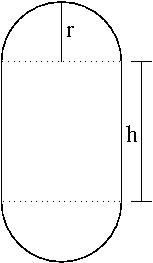
\includegraphics{corral-labeled.jpg}\end{image}



Then, we can note that \[A = h(2r)+\pi r^2.\] We also have the
constraint that there is only 800 feet of fencing available, so the
perimeter of the corral is
\[P = 2\pi r + 2h = 800 \Rightarrow \pi r +h = 400.\] Solving for $h$ we
have: \[h = 400-\pi r,\] so \begin{align*}
A &=  h(2r)+\pi r^2 \\
&= (400-\pi r)(2r) + \pi r^2 \\
&= 800r - \pi r^2 \\
A' &= 800 - 2\pi r \\
0 &= 800-2\pi r \\
r &= \frac{400}{\pi} \Rightarrow h = 400-\pi\left(\frac{400}{\pi}\right) = 400-400=0
\end{align*} In other words, the critical point of this area function occurs when
$r=400/\pi$ and $h=0$ so the corral is a circle. We can check that this
is a maximum using the second derivative test: \[A'' = -2\pi < 0 \] so
we are correct.

The area of the largest corral is
\[A = \pi \left(\frac{400}{\pi}\right)^2 = \frac{160000}{\pi} \mbox{ ft}^2.\]
\end{hint}


\begin{multipleChoice}
\choice{The largest possible corral is $40000\left(1+\frac{\pi}{4}\right)$
ft$^2$.}
\choice[correct]{The largest possible corral is $\frac{160000}{\pi}$.}
\choice{The largest possible corral is $800+\pi$ ft$^2$.}
\choice{The largest possible corral is $40000$ ft$^2$.}
\choice{The largest possible corral is 800 ft$^2$.}
\end{multipleChoice}

\end{exercise}
\end{document}
